\chapter{Methodology}

After analyzing the state-of-the-art, the following limitations were identified, which motivate the research presented in this thesis:
\begin{itemize}
    \item \textbf{Predefined roles for symbolic and subsymbolic models.} \cite{besold_neural-symbolic_2017} introduce a set of principles for neurosymbolic integration. One of the key aspects of this work is the distinction between representation and reasoning in neurosymbolic systems. This work denotes that symbolic models are used for representation, while subsymbolic models are used for reasoning. This statement is further validated by the work of \cite{garcez_neural-symbolic_2019}. The use of symbolic models as reasoning paradigms is therefore dismissed and not explored in the literature.
    
    \item \textbf{Integrations are mostly limited to rule-based systems and neural networks.} The AI spectrum, as outlined in Section \ref{sec:the_ai_spectrum}, comprises a wide variety of paradigms. In neurosymbolic systems, however, only rule-based systems and neural networks are featured, leaving a wide range of both symbolic and subsymbolic approaches unexplored. 
    
    \item \textbf{Limitations of neurosymbolic integration are not explored.} Most works in neurosymbolic design focus on the benefits or positive aspects derived from the integration of symbolic and subsymbolic models. The specific limitations that motivate certain neurosymbolic integrations are not outlined. This gives a biased perspective on the subject, as only presents the positive aspects of it.
    
    \item \textbf{Absence of guidelines on when and how neurosymbolic integration should be performed.} The most remarkable limitation is the absence of guidelines and case scenarios where neurosymbolic integration should be performed. Design proposals focus only on the representation and reasoning aspects of the integration, but do not consider potential issues such as computational costs, performance restrictions, or contextual elements. 
\end{itemize}


\section{Problem Statement} \label{3_sec:problem_statement}
This thesis presents a design method for hybrid learning models, focusing on the integration of knowledge-based systems (KBS) and deep learning (DL) models. Several neurosymbolic system categorizations were outlined in Section \ref{2_sec:subsec:categorization}, each focusing on a different aspect. This thesis proposes a categorization based on the integration mechanism: introduction and extraction. Introduction approaches combine KBS and DL models under a unified framework to perform a certain task. In extraction, one of the models is either mined or used to mine knowledge from the other. 

\begin{figure}[t]
    \centering
    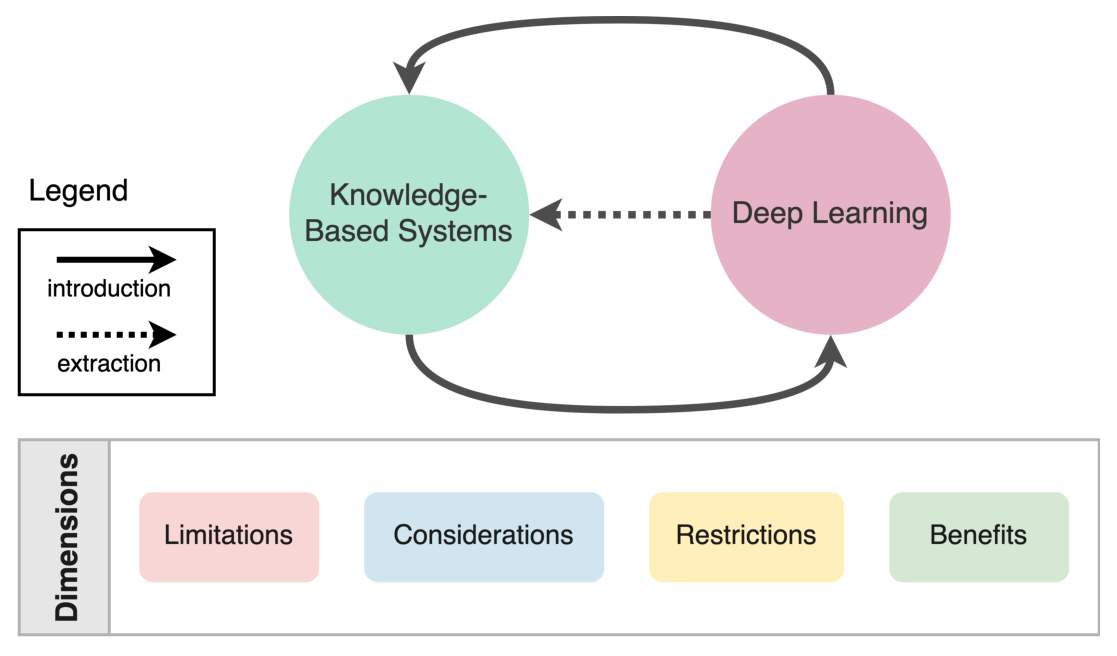
\includegraphics[width=.9\linewidth]{3_objectives/figures/overview_method.eps}
    \caption{Overview on the integration approaches and method design parameters proposed in this thesis.}
    \label{fig:thesis_overview}
\end{figure}

Figure \ref{fig:thesis_overview} showcases the three possible interactions between KBS and DL according to the aforementioned perspective: KBS injection in DL models, DL introduction into KBS, and KBS extraction from DL models. While the introduction is bidirectional, the extraction is only directed from DL to KBS. According to the provided definition for extraction, DL extraction from KBS would be unfeasible, and it is therefore not considered in this thesis. 

This thesis presents a general design method to model the three possible interactions between KBS and DL. Besides studying the potential benefits and the existing limitations of each model that motivate the integration, this method also contemplates previous requirements, as well as a set of criteria that must be met for the integration to be successful. The proposed design method comprises four dimensions, which are defined in a sequential order:
\begin{itemize}
    \item \textbf{Limitations.} Integration is motivated by the existence of limitations in one of the paradigms that could be resolved with the inclusion of a model from the opposite side of the spectrum. Limitations must be clearly identified before the integration. Model selection is based on the detected limitations and the goal of the system. This dimension only alludes to the model features.
    
    \item \textbf{Considerations.} Limitations must be framed into context. This dimension relates to the practical and contextual aspects of the integration. Infrastructural, user-related, and data aspects are depicted in this dimension.
    
    \item \textbf{Restrictions.} Integration carries an effort and serves a purpose. The effort made must not only be reflected in the results, but must also comply with a series of restrictions. Restrictions ensure that the integration not only is successful, but also that it is coherent and that the neurosymbolic system is justified for the given task and context.
    
    \item \textbf{Benefits.} A successful neurosymbolic integration entails a series of benefits. These benefits must be addressed in the context of the previously described limitations, and must be a direct result of the integration. This dimension should highlight the attainment of features that could not have been obtained otherwise.
\end{itemize}

\subsection{Research Hypotheses}
Once the research problem has been described, the following research hypotheses are formulated:
\begin{enumerate} [start=1,label={\bfseries H\arabic*:}]
    \item A general design method for the integration of knowledge-based systems and deep learning models can be proposed to accurately describe any hybrid learning model instance. 
    \item Knowledge-based systems and deep learning models are not antagonistic, but complimentary, and their integration can enable the resolution of problems that could not be achieved otherwise.
\end{enumerate}

\subsection{Goals}
As outlined in Section \ref{3_sec:problem_statement}, the main goal of this thesis is \textbf{to propose a general design method for the integration of knowledge-based systems and deep learning models.}  The proposed design method not only focuses on the motivation and benefits, but tackles the technical and contextual aspects that are needed to define a successful integration. For this purpose, two main objectives are defined:
\begin{enumerate}[start=1,label={\bfseries O\arabic*:}]
    \item Define a set of general parameters per dimension for the integration of knowledge-based systems and deep learning models.
    \item Instantiate the proposed design method across different models and use scenarios.
\end{enumerate}

\subsection{Contributions}
According to the proposed goals, the contributions can be grouped into two categories: interaction design methods and resources.
Regarding interaction design methods, the contributions are as follows:
\begin{enumerate}[start=1,label={\bfseries C\arabic*:}]
    \item Design method for the introduction of knowledge-based systems into deep learning models.
    \item Design method for the introduction of deep learning models into knowledge-based systems.
    \item Design method for knowledge-based system extraction from deep learning models.
\end{enumerate}
The design models depicted in contributions \textbf{C1,C2} and \textbf{C3} are instantiated on different use scenarios, generating the following resource contributions:
\begin{enumerate}[start=4,label={\bfseries C\arabic*:}]
    \item Semantic-based initialization method for knowledge graph embedding models.
    \item Modular case-based reasoning framework powered by deep learning models for document generation.
    \item Multi-agent system architecture for the extraction of behavioral patterns from black-box hyperpersonalization systems.
    \item GEnI: A framework for generating explanations and insights for knowledge graph embedding predictions
\end{enumerate}
\subsection{Assumptions}
The work in this thesis is developed under the following assumptions:
\begin{enumerate}[start=1,label={\bfseries A\arabic*:}]
    \item The proposed design method only considers the integration of knowledge-based systems and deep learning as described in Section \ref{sec:the_ai_spectrum}.
    \item Design parameters for each interaction may be updated if any of the reported limitations are solved without the need of integration.
    \item Instances based on the proposed design method comprise a continuous integration cycle, such that if one of the models change, this change must be extended to its counterpart
\end{enumerate}
\subsection{Restrictions}
The following restrictions limit the contributions of this thesis and may be used to lead future research works:
\begin{enumerate}[start=1,label={\bfseries R\arabic*:}]
    \item The design method presented in this thesis only applies to hybrid models \citep{hilario_overview_nodate} and modular models \citep{mcgarry_hybrid_1999}.
    \item The proposed design method only applies to integrations strictly between a knowledge-based system and a deep learning model. 
    \item On each interaction, one of the models plays a primary role while the other acts as a supporting (secondary) element.\\
    Note: In KBS extraction from DL models, the primary model is the one that performs the extraction, while the secondary is the one where the knowledge is extracted from.
    \item Design method instances do not need to comply with all the general parameters, but should at least comply with one parameter from each dimension. 
\end{enumerate}

Figure \ref{fig:methodology_general} depicts the hypotheses, goals, contributions, assumptions and restrictions, highlighting the relations between them. 

\begin{sidewaysfigure}
  \centering
  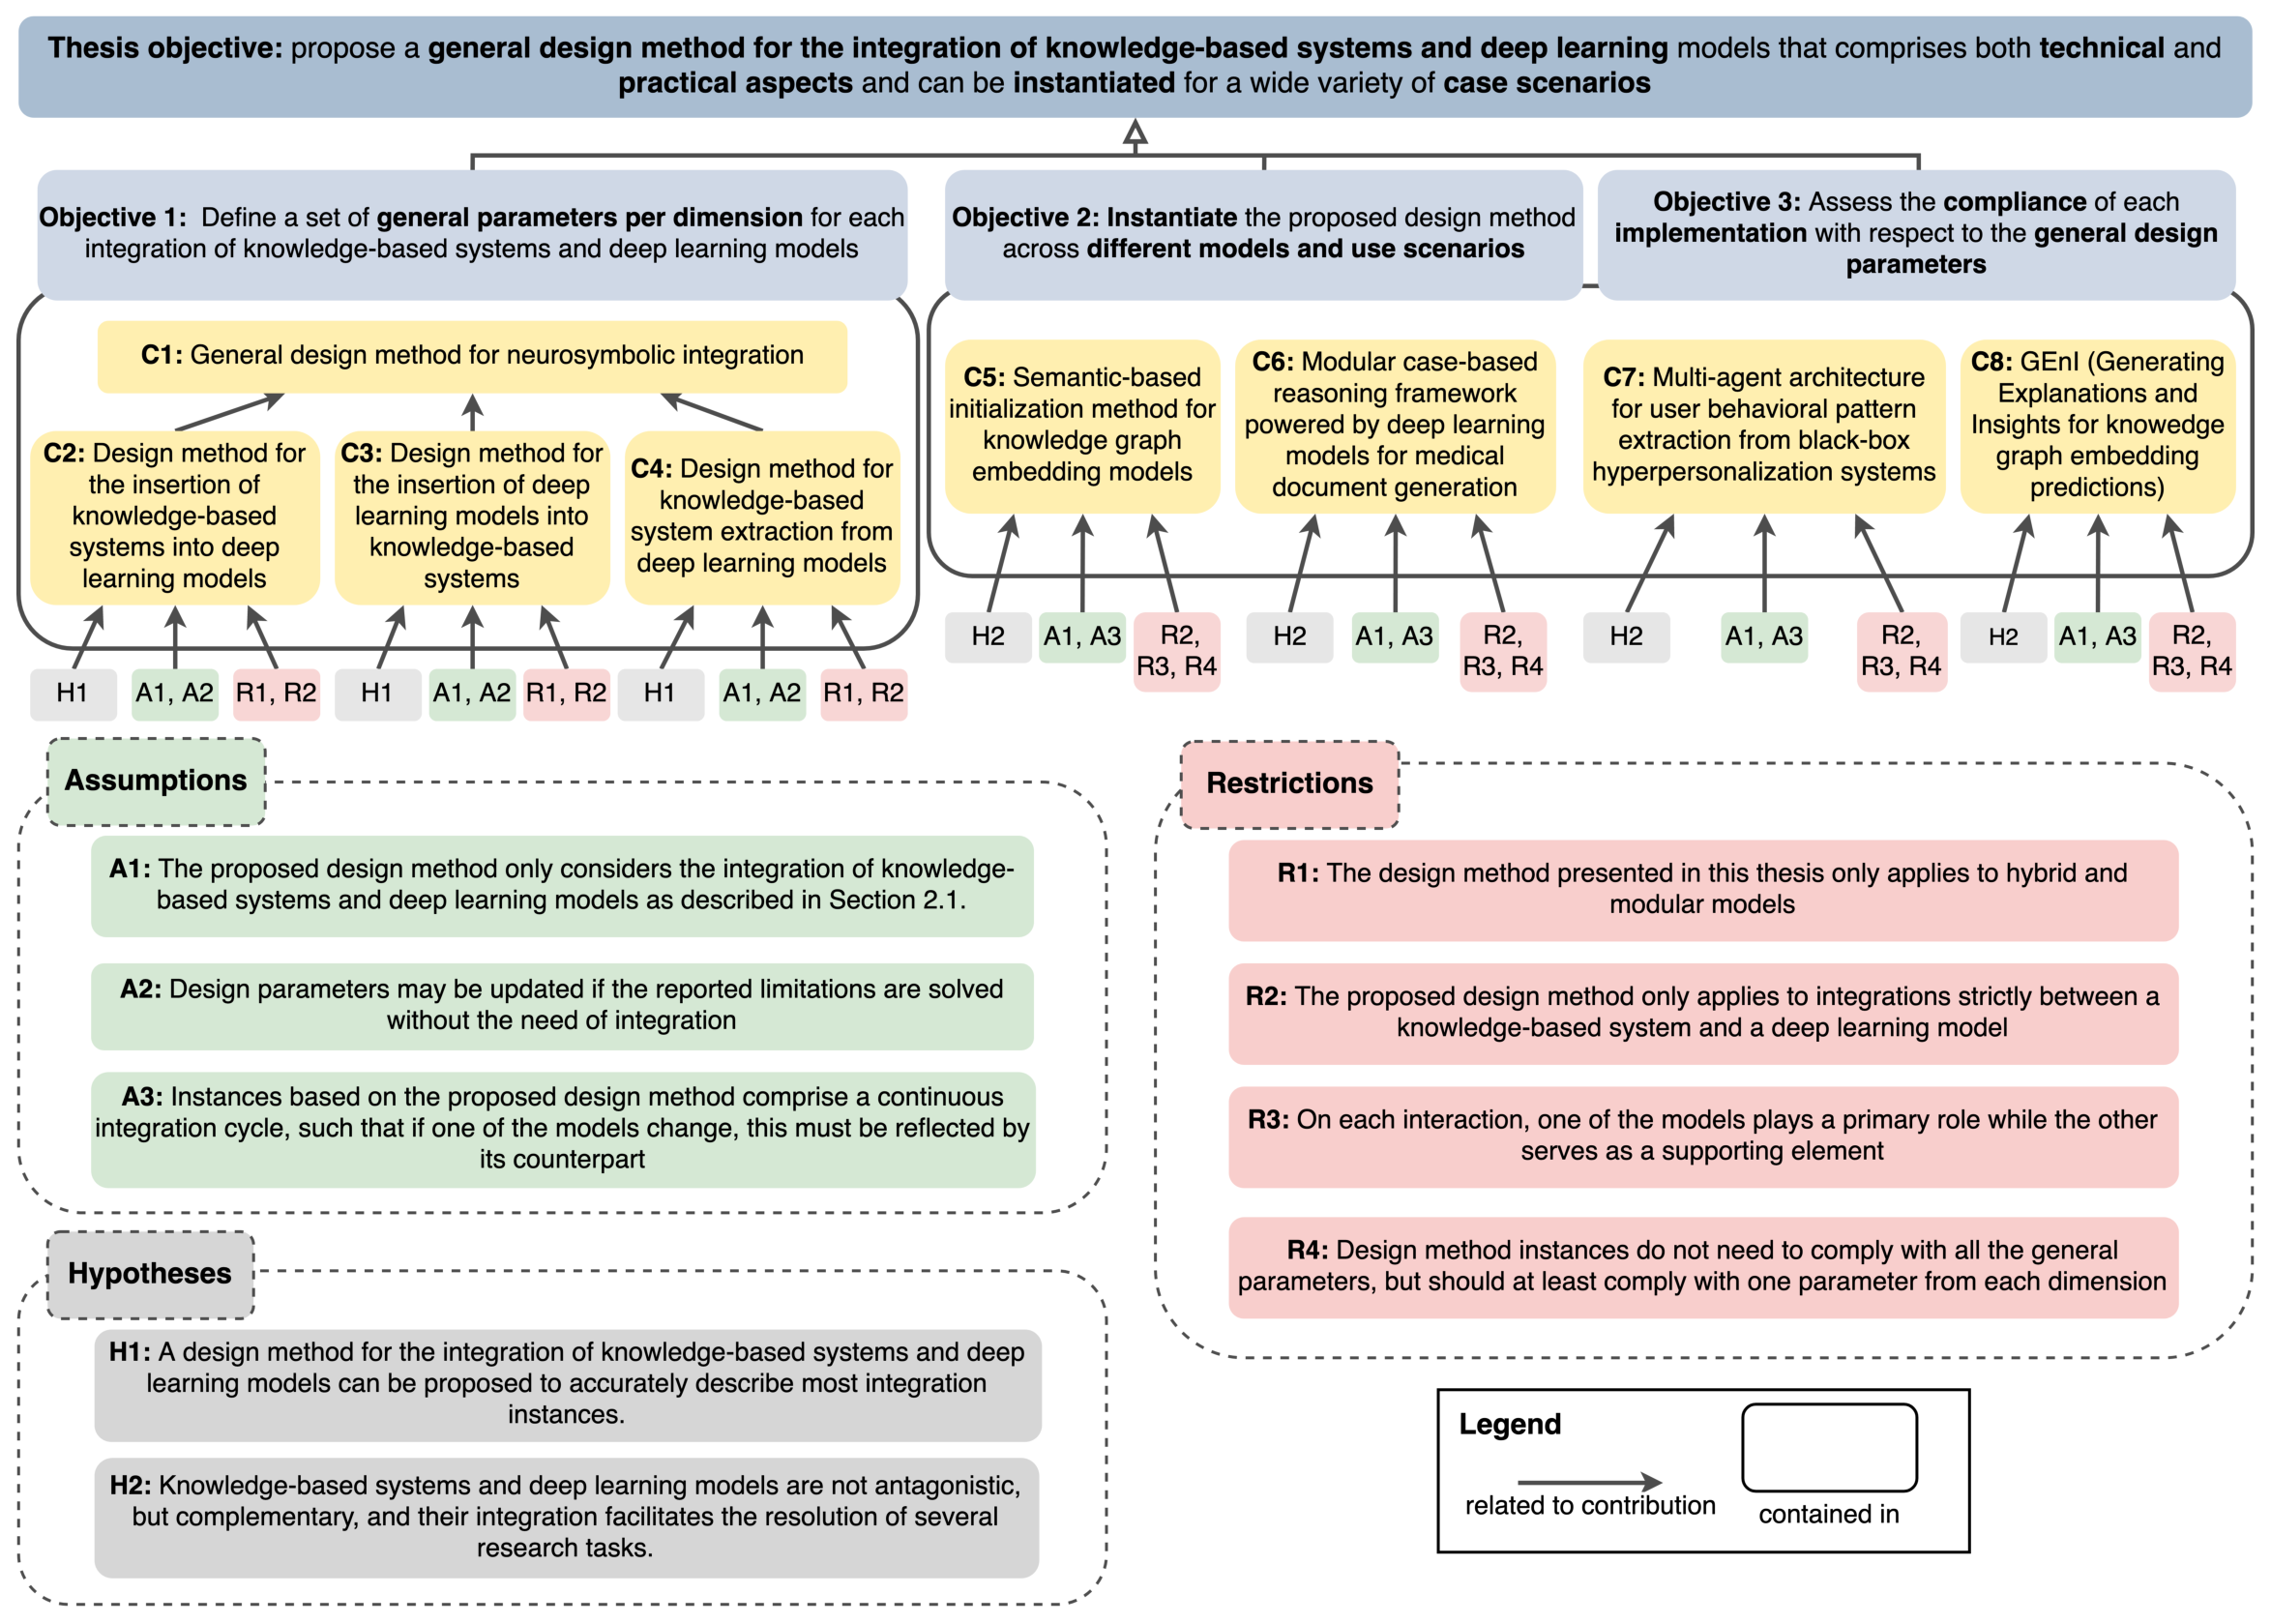
\includegraphics[width=\linewidth]{3_objectives/figures/methodology_general.eps}
  \caption{Correspondences between objectives, contributions, assumptions, hypotheses and restrictions.}
  \label{fig:methodology_general}
\end{sidewaysfigure}

\section{Research Methodology}\label{3_sec:research_methodology}
%%OBJETIVOS
% Definir los parámetros necesarios para llevar a cabo la integración de KBS y DL


%%ASSUMPTIONS
% Los métodos propuestos sólo consideran la integración de KBS y DL entendiendo como parte de estas categorías los modelos del SOTA en esta parte

% Los parámetros descritos pueden ser modificados en el futuro si las limitaciones existentes en alguno de los modelos fueran resueltas sin la necesidad de integración

%Se considera el proceso como un ciclo en el que si uno de los modelos cambia, el otro actua de manera acorde


%%RESTRICCIONES

%No consideramos modelos unificados donde ambos tienen la misma importancia, sino hibridos segun hilario (revisar notación para que sea coherente) o modulares segun mcgarry et al.

%existe un modelo maestro y un modelo 'slave'. No se puede usar esta terminologia ya porque es un poco reicist. Importante distinguir en integracion quien es el primary (EL QUE EJECUTA LA MAGRA) y el secondary (EL QUE MEJORA LA MAGRA). 

%En el caso de la extraccion, el primario es EL QUE EXTRAE y el secondary es DEL QUE SE EXTRAE.
 
%Importante diferenciar cuando se hace lo de la integracion de KBS a DL que se debe introducir INTERPRETABILIDAD.

%%Las instancias del método general no necesitan cumplir todos los parámetros generales, pero necesitan cumplir al menos un valor por parámetro.


%%%CONSIDERAMOS LOS METODOS DESDE CUATRO PERSPECTIVAS: LIMITACIONES, CONSIDERACIONES, CONSTRAINTS, IMPACTO.
